\subsubsection{Prescribed internal velocity constraints}
\label{sec:prescribed-velocities}
\textit{This section was contributed by Jonathan Perry-Houts}

In cases where it is desirable to investigate the behavior of one part of the model
domain but the controlling physics of another part is difficult to capture,
such as corner flow in subduction zones, it may be useful to force the desired
behavior in some parts of the model domain and solve for the resulting flow
everywhere else. This is possible through the use of \aspect{}'s ``signal'' mechanism,
as documented in Section~\ref{sec:extending-signals}.

Internally, \aspect{} adds ``constraints'' to the finite element system for boundary
conditions and hanging nodes. These are places in the finite element system where
certain solution variables are required to match some prescribed value. Although it
is somewhat mathematically inadmissible to prescribe constraints on nodes inside
the model domain, $\Omega$, it is nevertheless possible so long as the prescribed
velocity field fits in to the finite element's solution space, and satisfies the
other constraints (i.e., is divergence free).

Using \aspect{}'s signals mechanism, we write a shared library which provides a
``slot'' that listens for the signal which is triggered after the regular model
constraints are set, but before they are ``distributed.''

As an example of this functionality, below is a plugin which allows the user to prescribe
internal velocities with functions in a parameter file:
\lstinputlisting[language=C++]{../../cookbooks/prescribed_velocity/prescribed_velocity.cc}

The above plugin can be compiled with \texttt{cmake . \&\& make} in the
\url{cookbooks/prescribed_velocity} directory. It can be loaded in a parameter file
as an ``Additional shared library.'' By setting parameters like those shown below,
it is possible to produce many interesting flow fields such as the ones visualized in
(Figure~\ref{fig:prescribed-velocity}).
\lstinputlisting[language=prmfile]{minimal.prm.out}

\begin{figure}
    \centering
  \subfigure[]{
    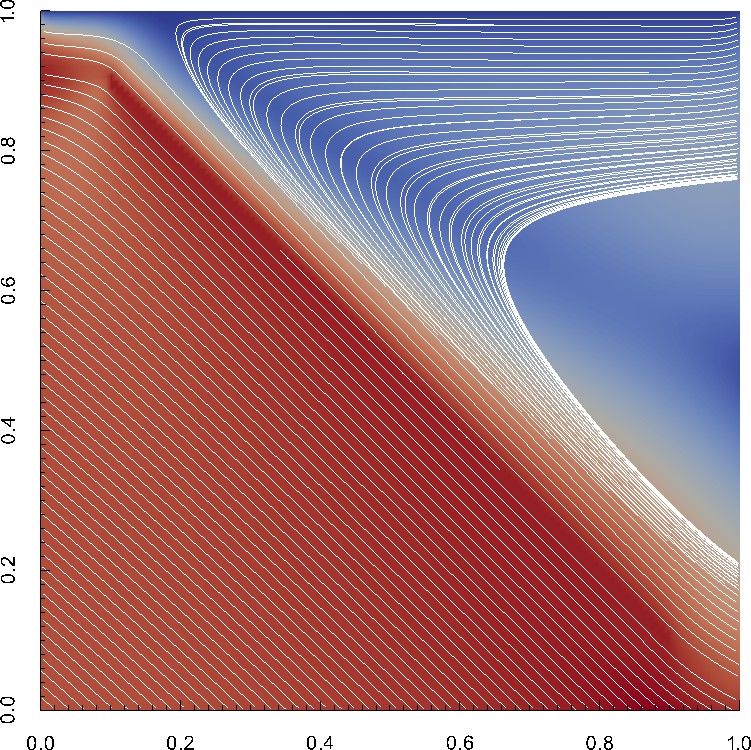
\includegraphics[width=.48\textwidth]{corner_flow.png}}
  ~
  \subfigure[]{
    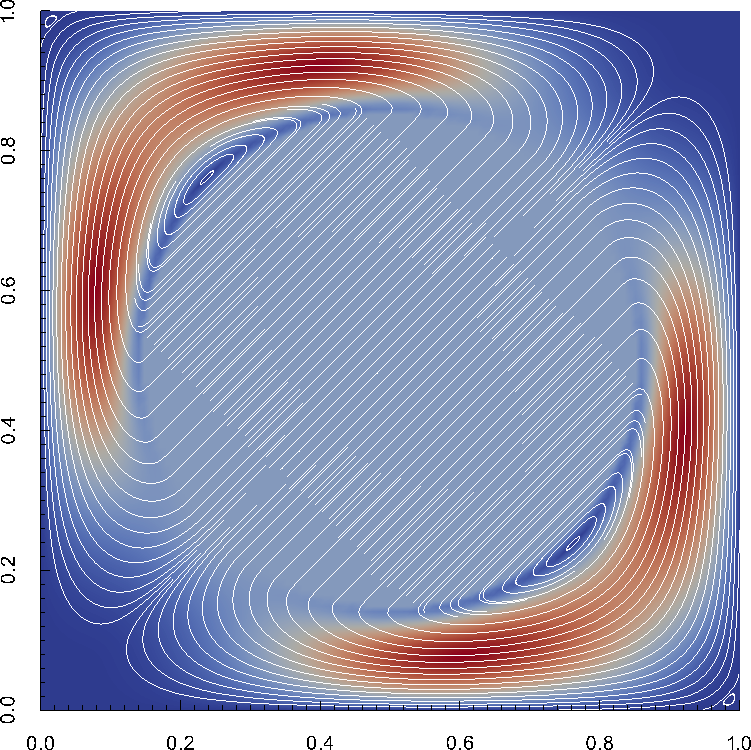
\includegraphics[width=.48\textwidth]{circle.png}}
    \caption{\it Examples of flows with prescribed internal velocities, as described in Section \ref{sec:prescribed-velocities}.}
    \label{fig:prescribed-velocity}
\end{figure}


